\providecommand{\tituloDocumento}{Evaluación}
\providecommand{\subtituloDocumento}{Función afín y sistemas de ecuaciones}

\documentclass{sn-guia}

\begin{document} 
\begin{tcbraster}[enhanced,raster columns=4,raster width=\linewidth,raster column skip=3pt,raster force size=false]
    \begin{caja}[title={\sffamily\scshape\bfseries Nombre},height=35pt,add to width=4.5cm]
    \end{caja}
    \begin{caja}[title={\sffamily\scshape\bfseries Curso},height=35pt,add to width=-1.5cm]
    \end{caja}    
    \begin{caja}[title={\sffamily\scshape\bfseries Puntaje},height=35pt,add to width=-1.5cm]
    \end{caja}
    \begin{caja}[title={\sffamily\scshape\bfseries Nota},height=35pt,add to width=-1.5cm]
    \end{caja}      
\end{tcbraster}
\vspace*{5mm}

\begin{problemas}
    \problema Considera la función $f$, cuyo dominio es el conjunto de los números reales,
    definida por $f(x)=2x-3$. ¿Cuál de los siguientes gráficos representa a la gráfica de $f$?
    \begin{alternativasgraficas}[]
        \grafica 
        \begin{tikzpicture}[scale=0.7]
            \draw[->] (0,0) -- (4,0) node [below] {$x$};
            \draw[->] (0,0) -- (0,5) node [left] {$y$};  
            \draw[line width=1pt] let \p{a} = (0,3), \p{b} = (2,1) in
                ($(\p{b})!1.5!(\p{a})$) -- ($(\p{a})!2!(\p{b})$);
            \node at (0,3) [left] {$3$};
            \node at (0,1) [left] {$1$};
            \node at (2,0) [below] {$2$};
            \draw[dashed] (0,1) -- (2,1) -- (2,0);
        \end{tikzpicture}
        \grafica 
        \begin{tikzpicture}[scale=0.7]
            \draw[->] (-4,0) -- (3,0) node [below] {$x$};
            \draw[->] (0,-1) -- (0,4) node [left] {$y$};  
            \draw[line width=1pt] let \p{a} = (-3,0), \p{b} = (2,1) in
                ($(\p{b})!1.15!(\p{a})$) -- ($(\p{a})!1.4!(\p{b})$);
            \node at (-3,0) [below] {$-3$};
            \node at (0,1) [left] {$1$};
            \node at (2,0) [below] {$2$};
            \draw[dashed] (0,1) -- (2,1) -- (2,0);
        \end{tikzpicture}  
        \grafica 
        \begin{tikzpicture}[scale=0.7]
            \draw[->] (0,0) -- (4,0) node [below] {$x$};
            \draw[->] (0,-4) -- (0,3) node [left] {$y$};  
            \draw[line width=1pt] let \p{a} = (0,-3), \p{b} = (2,1) in
                ($(\p{b})!1.2!(\p{a})$) -- ($(\p{a})!1.3!(\p{b})$);
            \node at (0,-3) [left] {$-3$};
            \node at (0,1) [left] {$1$};
            \node at (2,0) [below] {$2$};
            \draw[dashed] (0,1) -- (2,1) -- (2,0);
        \end{tikzpicture}
        \grafica 
        \begin{tikzpicture}[scale=0.7]
            \draw[->] (0,0) -- (4,0) node [below] {$x$};
            \draw[->] (0,-4) -- (0,3) node [left] {$y$};  
            \draw[line width=1pt] let \p{a} = (0,-3), \p{b} = (2,0) in
                ($(\p{b})!1.15!(\p{a})$) -- ($(\p{a})!1.4!(\p{b})$);
            \node at (0,-3) [left] {$-3$};
            \node at (2,0) [below] {$2$};
        \end{tikzpicture}      
    \end{alternativasgraficas}
    \problema Una empresa de mantención de equipos eléctricos cobra un costo fijo 
    mensual de \mbox{\$ 200.000} y \mbox{\$ 5.000} por cada visita que su técnico realice 
    en el mes. Si una fábrica contrata los servicios de esta empresa, ¿cuál de las siguientes 
    funciones modela el cobro total, en pesos, del servicio para $x$ visitas en el mes?
    \begin{alternativas}[]
        \alternativa $f(x) = 205.000x$
        \alternativa $f(x) = 200.000 -5.000x$
        \alternativa $f(x) = 200.000x + 5.000$
        \alternativa $f(x) = 5.000x + 200.000$
        \alternativa $f(x) = 5.000x - 200.000$
    \end{alternativas}
    \problema La suma de dos números es 42, donde la tercera parte del número mayor $(x)$
    más la mitad del número menor $(y)$ es igual al número menor. ¿Cúal de los siguientes 
    sistemas de ecuaciones lineales permite determinar los números?
    \begin{alternativasgraficas}[raster width=.5\textwidth]
        \grafica \begin{rcases}
            x + y &= 42 \\
            3x + \dfrac{y}{2} &= y
        \end{rcases}
        \grafica \begin{rcases}
            x &= 42 - y \\
            \dfrac{x}{3} + \dfrac{y}{2} &= y
        \end{rcases}
        \grafica \begin{rcases}
            y &= 42 + x \\
            3y + \dfrac{x}{2} &= x
        \end{rcases}
        \grafica \begin{rcases}
            x &= 42 + y \\
            \dfrac{x}{3} + \dfrac{y}{2} &= y
        \end{rcases}
    \end{alternativasgraficas} 
    
    \problema Una urna contiene en total 36 bolitas de dos tipos, $A$ y $B$. Cada bolita 
    del tipo $A$ tiene una masa de 100 g y cada bolita del tipo $B$ 150 g. Si la masa total
    de las bolitas en la urna es de 3.750 g, ¿Cuántas bolitas son del tipo $B$?
    \begin{alternativas}[]
        \alternativa 3
        \alternativa 12
        \alternativa 15
        \alternativa 18
        \alternativa 33
    \end{alternativas}
    
    \problema En el sistema de ecuaciones en $x$ e $y$:
    \begin{equation*}
        \begin{rcases*}
            px + qy &= p \\
            qx + py &= q 
        \end{rcases*},
    \end{equation*}
    donde $p$ y $q$ son números enteros positivos, ¿cuál(es) de las siguientes 
    afirmaciones es (son) verdadera(s)?
    \begin{enumerate}[label=\Roman*),leftmargin=2cm]
        \item Si $p=q$, entonces el sistema tiene infinitas soluciones.
        \item Si $p\neq q$, entonces el sistema tiene solución única.
        \item El sistema tiene una única solución.
    \end{enumerate}
    \begin{alternativas}[]
        \alternativa Solo I
        \alternativa Solo II
        \alternativa Solo III
        \alternativa Solo I y II
        \alternativa Solo II y III
    \end{alternativas}

    \problema Una compañia de agua potable cobra un cargo fijo mensual de $b$, además de 
    $m$ por cada metro cúbico de agua consumido en el mes. 
    Si $m\neq b$, ¿Cuál de las siguientes gráficas representa mejor la relación 
    entre los metros cubicos consumidos $(x)$ y el cobro mensual $f(x)$?
    \begin{alternativasgraficas}[raster columns=3]
        \grafica \begin{tikzpicture}[scale=0.5]
            \draw[->] (0,0) -- (0,5) node [left] {$f(x)$};
            \draw[->] (0,0) -- (5,0) node [below] {$x$};
            \draw[line width=1pt] (1,0) node [below] {$b$} -- ++(30:5);
        \end{tikzpicture}
        \grafica \begin{tikzpicture}[scale=0.5]
            \draw[->] (0,0) -- (0,5) node [left] {$f(x)$};
            \draw[->] (0,0) -- (5,0) node [below] {$x$};
            \draw[line width=1pt] (1,0) node [below] {$m$} -- ++(30:5);
        \end{tikzpicture}
        \grafica \begin{tikzpicture}[scale=0.5]
            \draw[->] (0,0) -- (0,5) node [left] {$f(x)$};
            \draw[->] (0,0) -- (5,0) node [below] {$x$};
            \draw[line width=1pt] (0,1) node [left] {$m$} -- ++(30:5);
        \end{tikzpicture}
        \grafica \begin{tikzpicture}[scale=0.5]
            \draw[->] (0,0) -- (0,5) node [left] {$f(x)$};
            \draw[->] (0,0) -- (5,0) node [below] {$x$};
            \draw[line width=1pt] (0,1) node [left] {$b$} -- ++(30:5);
        \end{tikzpicture}
        \grafica \begin{tikzpicture}[scale=0.5]
            \draw[->] (0,0) -- (0,5) node [left] {$f(x)$};
            \draw[->] (0,0) -- (5,0) node [below] {$x$};
            \draw[line width=1pt] (0,0) -- ++(30:5) coordinate[midway] (P);
            \draw[dashed] (P) -- (P-|{(0,0)}) node [left] {$b$};
            \draw[dashed] (P) -- (P|-{(0,0)}) node [below] {$1$};
        \end{tikzpicture}
    \end{alternativasgraficas}
    \problema El par de números $x=3/2$ e $y=-3/2$ son solución del sistema:
    \begin{equation*}
        \begin{rcases*}[]
            ax - y &= 6 \\
            x - by &= 6
        \end{rcases*}.
    \end{equation*}
    El valor de $(a+b)$ es 
    \begin{alternativas}[]
        \alternativa 3
        \alternativa 0
        \alternativa 6
        \alternativa 2
        \alternativa 10
    \end{alternativas}

    \problema 
    Alberto entra a una librería con el objetivo de gastar exaxtamente \mbox{\$ 100.000} 
    en comprar 70 lápices. En la librería tienen solo dos tipos de lápices, uno vale 
    \mbox{\$ 1.500} y el otro vale \mbox{\$ 1.200}. ¿Cuántos lápices de cada tipo debe
    comprar en la librería, para cumplir su objetivo?
    \begin{alternativas}
        \alternativa 53 y 17
        \alternativa 54 y 16
        \alternativa 53 y 16
        \alternativa Otras cantidades.
        \alternativa Alberto no puede complir su objetivo.
    \end{alternativas}

    \problema ¿Cuál de los siguientes sistemas tiene una única solución?
    \begin{alternativasgraficas}[raster columns=3]
        \grafica \begin{rcases}
            4x - 3y + 2 &= 0 \\
            x - \dfrac{3}{4}y &= -\dfrac{1}{2}
        \end{rcases}
        \grafica \begin{rcases}
            7x - y &= 7 \\
            y - 7x &= 32
        \end{rcases}
        \grafica \begin{rcases}
            x &= 8 \\
            y - x &= 0
        \end{rcases}
        \grafica \begin{rcases}
            2x - y &= 6 \\
            -4x + 2y + 12 &= 0
        \end{rcases}
        \grafica \begin{rcases}
            x - y &= 10 \\
            \dfrac{1}{5}x - \dfrac{1}{5}y &= 2
        \end{rcases}
    \end{alternativasgraficas}
    \problema Dos variables $x$ y $z$ dependen entre sí según la ecuación $z = ax +c$. La
    tabla adjunta muestra algunos de los valores de $x$ y $z$. ¿Cuáles son los valores de 
    $a$ y $c$, respectectivamente?
    \begin{center}
        \vspace*{10pt}
        \begin{mtabla}{c|c}
            $x$ & $z$ \\
            1   & 4     \\
            2   & 6,5   \\
        \end{mtabla}
        \vspace*{10pt}
    \end{center}
    \begin{alternativas}
        \alternativa \begin{tblr}{colspec={X[r]X[r]X[r]},width=0.19\textwidth} $5$ & y & $\dfrac{3}{2}$ \end{tblr}
        \alternativa \begin{tblr}{colspec={X[r]X[r]X[r]},width=0.19\textwidth} $\dfrac{21}{2}$ & y & $-\dfrac{13}{2}$ \end{tblr}
        \alternativa \begin{tblr}{colspec={X[r]X[r]X[r]},width=0.19\textwidth} $-\dfrac{2}{5}$ & y & $\dfrac{22}{5}$ \end{tblr}
        \alternativa \begin{tblr}{colspec={X[r]X[r]X[r]},width=0.19\textwidth} $\dfrac{5}{2}$ & y & $\dfrac{3}{2}$ \end{tblr}
        \alternativa \begin{tblr}{colspec={X[r]X[r]X[r]},width=0.19\textwidth} $\dfrac{2}{5}$ & y & $-\dfrac{3}{5}$ \end{tblr}
    \end{alternativas}

    \problema El precio de un artículo es \$ M, el cual es cancelado con 16 monedas de dos 
    tipos, $x$ de un tipo e $y$ del otro tipo, cuyos valores son de \mbox{\$ $p$} y 
    \mbox{\$ $q$}, respectivamente. ¿Cuál de los siguientes sistemas, al resolverlo, 
    da como solución {\bfseries siempre} la cantidad de monedas de cada valor utilizadas
    para cancelar el artículo?
    \begin{alternativasgraficas}[raster columns=2,raster width=0.7\textwidth]
        \grafica \begin{rcases}
            (p+q)\cdot(x+y) &= M \\
            x+y &= 16
        \end{rcases}
        \grafica \begin{rcases}
            px + qy &= M \\
            (p+q)\cdot(x+y) &= 16
        \end{rcases}
        \grafica \begin{rcases}
            xp + yq &= M \\
            x + y &= 16
        \end{rcases}
        \grafica \begin{rcases}
            x + y &= M \\
            xp + yq &= 16
        \end{rcases}
        \grafica \begin{rcases}
            p + q &= M(x+y) \\
            xp + yq &= 16
        \end{rcases}
    \end{alternativasgraficas}
    \problema Una bomba comienza a llenar con agua un estanque cilíndrico de base horizontal
    y plana, a caudal constante. Si inicialmente el estanque contenía \mbox{2 $\text{m}^3$}
    de agua, ¿cuál de los siguientes gráficos representa mejor la altura $h(t)$, en m, 
    que alcanza el nivel de agua en el estanque, después de $t$ segundos desde que se 
    comenzó a llenar?
    \begin{alternativasgraficas}[raster columns=3]
        \grafica 
        \begin{tikzpicture}[scale=0.6]
            \draw[->] (0,0) -- (0,5) node [left] {$h(t)$};
            \draw[->] (0,0) -- (5,0) node [below] {$t$};
            \draw[line width=1pt] (0,0) -- ++(60:4);
        \end{tikzpicture} 
        \grafica 
        \begin{tikzpicture}[scale=0.6]
            \draw[->] (0,0) -- (0,5) node [left] {$h(t)$};
            \draw[->] (0,0) -- (5,0) node [below] {$t$};
            \draw[line width=1pt] (0,2) to [out=70, in=180] (3,4);
        \end{tikzpicture} 
        \grafica 
        \begin{tikzpicture}[scale=0.6]
            \draw[->] (0,0) -- (0,5) node [left] {$h(t)$};
            \draw[->] (0,0) -- (5,0) node [below] {$t$};
            \draw[line width=1pt] (2,0) -- ++(60:4);
        \end{tikzpicture} 
        \grafica 
        \begin{tikzpicture}[scale=0.6]
            \draw[->] (0,0) -- (0,5) node [left] {$h(t)$};
            \draw[->] (0,0) -- (5,0) node [below] {$t$};
            \draw[line width=1pt] (0,2) -- ++(60:4);
        \end{tikzpicture} 
        \grafica 
        \begin{tikzpicture}[scale=0.6]
            \draw[->] (0,0) -- (0,5) node [left] {$h(t)$};
            \draw[->] (0,0) -- (5,0) node [below] {$t$};
            \draw[line width=1pt] (0,2) to [out=0, in=270] (3,4);
        \end{tikzpicture} 
    \end{alternativasgraficas}
    
    \problema Ignacio se dedica a vender productos encargados por sus clientes, 
    que importa mediante una aplicación móvil. El precio de venta al que Ignacio 
    vende los productos lo determina según la función $P(x)=1,5x+2500$, tal que $x$
    representa el precio, en pesos, al que compra el producto en la aplicación.

    ¿Cuál de las siguientes afirmaciones es verdadera?
    \begin{alternativas}
        \alternativa Ignacio cobra un costo fijo de \$ $(1,5 + 2500)$ a todos los
        productos que vende.
        \alternativa Ignacio realiza un recargo de un 50 \% del precio del 
        producto importado sin considerar ese recargo en el cargo fijo.
        \alternativa Ignacio cobra un costo fijo de \$ $(1,5\cdot 2500)$ a todos
        los productos que vende.
        \alternativa Ignacio realiza un recargo de 1,5 \% del precio del producto 
        importado sin considerar el cargo fijo.
    \end{alternativas}
    
    \problema En el gráfico adjunto, se muesta la distancia en kilómetos recorrida 
    por 4 camiones ($A$, $B$, $C$ y $D$) durante un período de tiempo. ¿Cuál(es) 
    de las siguientes afirmaciones es (son) verdadera(s)?
    \begin{tcolorbox}[blanker,sidebyside,lefthand ratio=0.6]
    \begin{enumerate}[leftmargin=2cm,label=\Roman*)]\raggedright
        \item El camión $D$ es el más rapido.
        \item El camión $C$ recorre dos veces la distancia que recorre el camión $A$.
        \item El camión $B$ recorre la mitad de la distancia que recorre el 
        camión $D$.
    \end{enumerate}
    \begin{alternativas}
        \alternativa Solo I
        \alternativa Solo II
        \alternativa Solo III
        \alternativa Solo I y II
        \alternativa Solo I y III
    \end{alternativas}
    \tcblower
        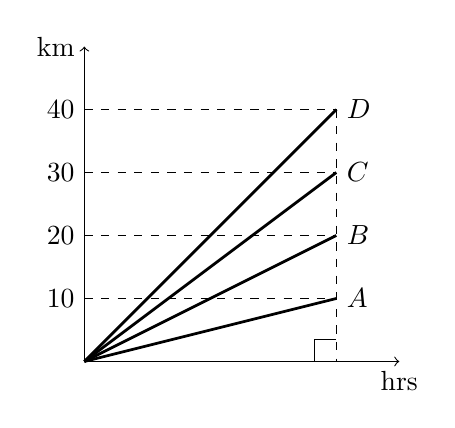
\begin{tikzpicture}[scale=0.8]
            \draw[->] (0,0) -- (0,5) node [left] {km};
            \draw[->] (0,0) -- (5,0) node [below] {hrs};
            \draw[line width=1pt] (0,0) -- (4,1) node [right] {$A$}; 
            \draw[line width=1pt] (0,0) -- (4,2) node [right] {$B$}; 
            \draw[line width=1pt] (0,0) -- (4,3) node [right] {$C$}; 
            \draw[line width=1pt] (0,0) -- (4,4) node [right] {$D$};
            \draw[dashed] (0,4) node [left] {40} -- (4,4); 
            \draw[dashed] (0,3) node [left] {30} -- (4,3); 
            \draw[dashed] (0,2) node [left] {20} -- (4,2); 
            \draw[dashed] (0,1) node [left] {10} -- (4,1);
            \draw[dashed] (4,4) -- (4,0);
            \draw (4,0) -- ++(180:10pt) -- ([turn]-90:10pt) -- ([turn]-90:10pt); 
        \end{tikzpicture}
    \end{tcolorbox}
    \problema ¿Cuál(es) de los siguientes gráficos podría(n) representar a una recta de
    ecuación $y=ax-3$?
    \begin{alternativasgraficas}[title={\RNum{\thetcbrasternum})},raster columns=3]
        \grafica 
        \begin{tikzpicture}[x=0.7cm,y=0.5cm]
            \draw[->] (-1,0) -- (4,0) node [below] {$x$};
            \draw[->] (0,-4) -- (0,2) node [left] {$y$};
            \draw[line width=1pt] let \p{c} = (0,-3) in
                (\p{c}) -- +(225:1) (\p{c}) node [right] {$-3$} -- +(45:5);
        \end{tikzpicture}
        \grafica 
        \begin{tikzpicture}[x=0.7cm,y=0.5cm]
            \draw[->] (-4,0) -- (1,0) node [below] {$x$};
            \draw[->] (0,-4) -- (0,2) node [left] {$y$};            
            \draw[line width=1pt] let \p{c} = (0,-3) in
                (\p{c}) -- +(135:5) (\p{c}) node [right] {$-3$} -- +(315:1);
        \end{tikzpicture}
        \grafica 
        \begin{tikzpicture}[x=0.7cm,y=0.5cm]
            \draw[->] (-4,0) -- (1,0) node [below] {$x$};
            \draw[->] (0,-2) -- (0,4) node [left] {$y$};
            \draw[line width=1pt] let \p{c} = (0,3) in
                (\p{c}) -- +(45:1) (\p{c}) node [right=5pt] {$3$} -- +(225:5);
        \end{tikzpicture}
    \end{alternativasgraficas}
    \begin{alternativas}
        \alternativa Solo I
        \alternativa Solo II
        \alternativa Solo III
        \alternativa Solo I y II
        \alternativa Ninguno de ellos.
    \end{alternativas}

    \problema En un cajón solo hay fichas blancas y rojas. De estas, $m$ son blancas y 
    $4n$ son rojas. Si se saca la mitad de las fichas blancas, entonces el cajón queda con un
    total de 110 fichas. En cambio, si se agrega un 75\% del total de fichas blancas y se
    quitan 10 fichas rojas, entonces el cajón queda con un total de 175 fichas. ¿Cuál es 
    el total de fichas que había inicialmente en el cajón?
    \begin{alternativas}
        \alternativa 80
        \alternativa 101
        \alternativa 73
        \alternativa 140
        \alternativa Ninguno de los valores anteriores.
    \end{alternativas}

    \problema Una compañia distribuidora de energía eléctrica cobra mensualmente un cargo
    fijo de \mbox{\$ 1.100} y \mbox{\$ 65} por kWh de consumo, pero si en los meses de invierno se superan
    los 200 kWh, se aplica un recargo de \$ 50 por cada kWh de exceso.
    
    ¿Cuál de las siguientes funciones permite calcular el total que se debe pagar en un mes
    de invierno por $x$ kWh si $x$ es mayor que 200?
    \begin{alternativas}
        \alternativa $f(x) = 1.100 + (200\cdot 65) + 50x$
        \alternativa $f(x) = 1.100 + (200\cdot 65) + 115x$
        \alternativa $f(x) = 1.100 + 115x$
        \alternativa $f(x) = 1.100 + (200\cdot 65) + 115(x-200)$
    \end{alternativas}
    
    \problema Si se supone que un modelo para la temperatura $T$, en grados Celsius (°C),
    de un líquido recién vertido en un recipiente está dado por $T(t) = 90 - 10t$, donde $t$
    es el tiempo transcurrido en minutos, desde el instante en que fue vertido, ¿cuál(es) de
    las siguientes afirmaciones es (son) verdadera(s)?

    \begin{enumerate}[label=\Roman*),leftmargin=2cm]
        \item La temperatura disminuye en función del tiempo.
        \item El líquido fue vertido a 90 °C.
        \item La temperatura del líquido disminuye a razón de 10 °C por minuto
    \end{enumerate}
    \begin{alternativas}
        \alternativa Solo I
        \alternativa Solo II
        \alternativa Solo I y III
        \alternativa Solo II y III
        \alternativa I, II y III
    \end{alternativas}

    \problema Un paciente evalúa costos en dos posibles centros de terapía, $M$ y $P$. En 
    $M$ paga 1 UF por el contrato más 0,5 UF por cada sesión de terapia y en P paga 2/3 UF
    por cada sesión de terapía. ¿Cuál de las siguientes afirmaciones es verdadera?

    \begin{alternativas}
        \alternativa Es más conveniente el centro $M$, independiente del número de sesiones.
        \alternativa Si decide contratar 4 sesiones de terapía, entonces debería optar por
        el centro $M$, que es el más conveniente.
        \alternativa Las variables número de sesiones y costo asociado, para el 
        centro $M$, son directamente proporcionales.
        \alternativa Para un tratamiento de 6 sesiones se pagaría 4 UF en cualquiera 
        de los centros de terapia. 
        \alternativa Es más conveniente el centro $P$, independiente del número de sesiones.
    \end{alternativas}

    \problema 
    Un cargador de celular del tipo $A$ carga \mbox{1 \%} de la capacidad de la batería cada 
    3 minutos y un cargador de tipo $B$ carga \mbox{1 \%} de la capacidad de la batería cada 
    2 minutos. 
    
    Se tienen dos celulares de las mismas caracteristicas. Uno tiene un \mbox{20 \%} de 
    batería cargada y se conecta al cargador del tipo $A$, mientras que el otro 
    celular tiene un \mbox{15 \%} de su batería cargada y se conecta al cargador del tipo
    $B$.

    ¿Cuál de los siguientes gráficos representa de mejor manera el porcentaje de carga
    de las baterías a medida que transcurren los minutos?
    \begin{alternativasgraficas}
        \grafica 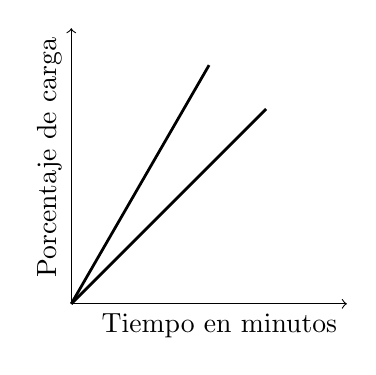
\begin{tikzpicture}[scale=0.7]
            \draw[->] (0,0) -- (5,0) node [below,anchor=north east] {Tiempo en minutos};
            \draw[->] (0,0) -- node [at end,sloped,above,anchor=south east] 
                {Porcentaje de carga} (0,5);
            \draw[line width=1pt] (0,0) -- (45:5);
            \draw[line width=1pt] (0,0) -- (60:5);
        \end{tikzpicture}
        \grafica 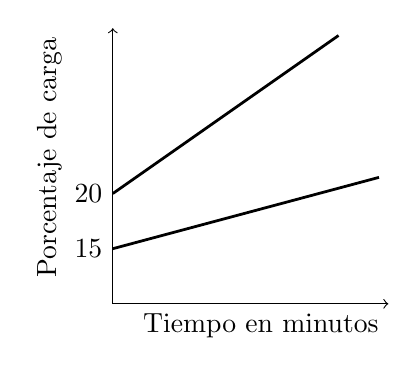
\begin{tikzpicture}[scale=0.7]
            \draw[->] (0,0) -- (5,0) node [below,anchor=north east] {Tiempo en minutos};
            \draw[->] (0,0) -- node [at end,sloped,above=15pt,anchor=south east] 
                {Porcentaje de carga} (0,5);
            \draw[line width=1pt] (0,2) node[left]{20} -- +(35:5);
            \draw[line width=1pt] (0,1) node[left]{15} -- +(15:5);
        \end{tikzpicture}
        \grafica 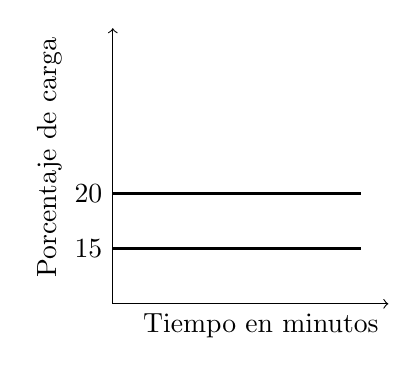
\begin{tikzpicture}[scale=0.7]
            \draw[->] (0,0) -- (5,0) node [below,anchor=north east] {Tiempo en minutos};
            \draw[->] (0,0) -- node [at end,sloped,above=15pt,anchor=south east] 
                {Porcentaje de carga} (0,5);
            \draw[line width=1pt] (0,2) node[left]{20} -- (4.5,2);
            \draw[line width=1pt] (0,1) node[left]{15} -- (4.5,1);
        \end{tikzpicture}
        \grafica 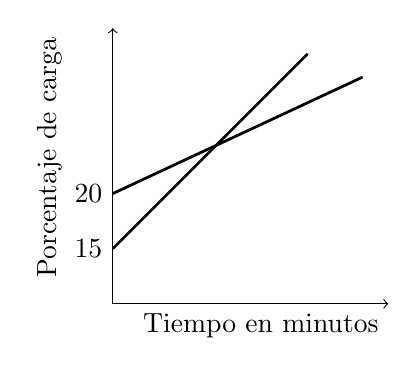
\begin{tikzpicture}[scale=0.7]
            \draw[->] (0,0) -- (5,0) node [below,anchor=north east] {Tiempo en minutos};
            \draw[->] (0,0) -- node [at end,sloped,above=15pt,anchor=south east] 
                {Porcentaje de carga} (0,5);
            \draw[line width=1pt] (0,1) node[left]{15} -- +(45:5);
            \draw[line width=1pt] (0,2) node[left]{20} -- +(25:5);
        \end{tikzpicture}
    \end{alternativasgraficas}

    \problema Un vehículo ha recorrido $pq$ kilómetros, donde $p$ es el dígito de las 
    decenas y $q$ el dígito de las unidades. La suma de los dígitos que componen dicho 
    número es ocho. Dieciocho kilómetros más adelante ha recorrido $qp$ kilómetros,
    donde $q$ es el dígito de las decenas y $p$ el dígito de las unidades. ¿Cuál de los
    siguientes sistemas permite determinar los kilómetros recorridos?
    \begin{alternativasgraficas}[raster columns=3]
        \grafica \begin{rcases}
            p + q &= 8 \\
            p + q &= 10q + p - 18
        \end{rcases}
        \grafica \begin{rcases}
            p + q &= 8 \\
            10q + p &= 10p + q + 18
        \end{rcases}
        \grafica \begin{rcases}
            p + q &= 8 \\
            p + q  - 18 &= 10p + q
        \end{rcases}
        \grafica \begin{rcases}
            p + q &= 8 \\
            10q + p + 18 &= 10p + q
        \end{rcases}
        \grafica \begin{rcases}
            p + q &= 8 \\
            p + q + 18 &= 10p + q
        \end{rcases}
    \end{alternativasgraficas}

    \problema Una persona controla un dron y comienza a hacerlo decender verticalmente con 
    una rapidez constante de 5 metros por segundo. 

    Si al momento de iniciar el descenso el dron se encontraba a una altura de 80 metros
    con respecto al suelo, ¿cuál de los siguientes gráficos representa mejor la altura 
    del dron con respecto al suelo, a medida que transcurre el tiempo, en segundos, desde
    el inicio del descenso?
    \begin{alternativasgraficas}
        \grafica 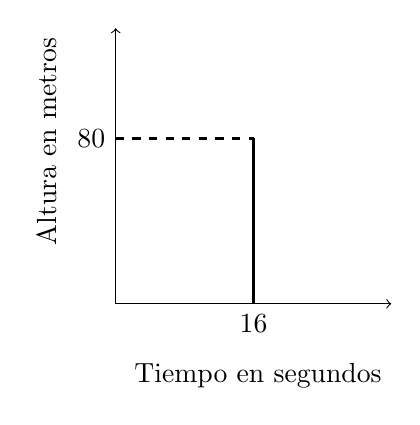
\begin{tikzpicture}[scale=0.7]
            \draw[->] (0,0) -- (5,0) node [below=18pt,anchor=north east] {Tiempo en segundos};
            \draw[->] (0,0) -- node [at end,sloped,above=18pt,anchor=south east] 
                {Altura en metros} (0,5);
            \draw [line width=1pt,dashed] (0,3) node [left]{80} -- (2.5,3);
            \draw [line width=1pt] (2.5,3) -- (2.5,0) node[below]{16};
        \end{tikzpicture}
        % \begin{tikzpicture}
        %     \begin{axis}[axis lines=left,axis line style={->},axis lines=center,width=6cm,
        %         xlabel=Tiempo en segundos, ylabel=Altura en metros,
        %         xtick={16}, ytick={80},xmin=0,xmax=50,ymin=0,ymax=100,
        %         xlabel style = {at={(axis description cs:1,0)},anchor=north east,yshift=-18pt},
        %         ylabel style = {at={(axis description cs:0,1)},anchor=south east,rotate=90,yshift=18pt}]
        %         %\addplot+ [samples=3,domain=-1:3] {x};
        %         \addplot[line width=1pt] coordinates {(16,0) (16,80)};
        %         \draw[dashed] (0,80) -- (16,80);
        %     \end{axis}
        % \end{tikzpicture}
        \grafica 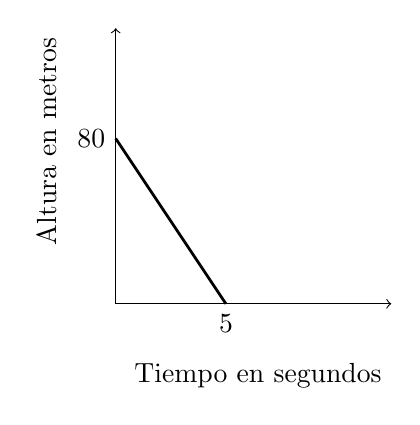
\begin{tikzpicture}[scale=0.7]
            \draw[->] (0,0) -- (5,0) node [below=18pt,anchor=north east] {Tiempo en segundos};
            \draw[->] (0,0) -- node [at end,sloped,above=18pt,anchor=south east] 
                {Altura en metros} (0,5);
            \draw [line width=1pt] (2,0) node [below]{5} -- (0,3) node[left]{80};
        \end{tikzpicture}
        \grafica 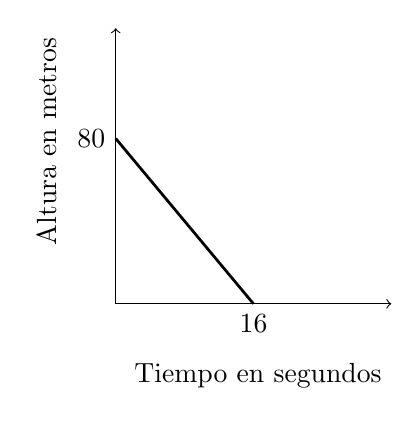
\begin{tikzpicture}[scale=0.7]
            \draw[->] (0,0) -- (5,0) node [below=18pt,anchor=north east] {Tiempo en segundos};
            \draw[->] (0,0) -- node [at end,sloped,above=18pt,anchor=south east] 
                {Altura en metros} (0,5);
            \draw [line width=1pt] (0,3) node [left]{80} -- (2.5,0)
                node[below]{16};
        \end{tikzpicture}
        \grafica 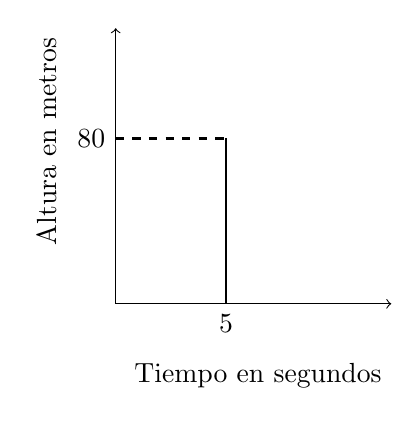
\begin{tikzpicture}[scale=0.7]
            \draw[->] (0,0) -- (5,0) node [below=18pt,anchor=north east] {Tiempo en segundos};
            \draw[->] (0,0) -- node [at end,sloped,above=18pt,anchor=south east] 
                {Altura en metros} (0,5);
            \draw [line width=1pt,dashed] (0,3) node [left]{80} -- (2,3);
            \draw [line width=1pt] (2,3) -- (2,0) node[below]{5};
        \end{tikzpicture}
    \end{alternativasgraficas}

    \problema Dado el sistema 
    \begin{equation*}
        \begin{rcases*}
            mx + ny &= 9 \\
            3mx - ny &= 7
        \end{rcases*},
    \end{equation*}
    en $x$ e $y$, con $m$ y $n$ distintos de 0 y distintos entre sí, ¿cuál de las siguientes
    expresiones representa el valor de $(mn(x+y))$?
    \begin{alternativas}
        \alternativa $5m+4n$
        \alternativa $m+8n$
        \alternativa $4m+5n$
        \alternativa $10m-n$
        \alternativa $13m+4n$
    \end{alternativas}
\end{problemas}

\vspace*{\fill}
\begin{center}
    \begin{tikzpicture}[ampersand replacement=\&,]
        %\node (A) [opacity=0.4] {\includegraphics[width=2cm]{../flork3.jpg}};
        \node (B) [font=\slshape,text width=12cm]
        {``Cree en ti mismo y en lo que eres. Sé consciente de que hay algo en tu interior %
        que es más grande que cualquier obstáculo''};
        \node [left=0mm of B,opacity=0.4] {\pgfornament[width=2cm]{37}};
        \node [right=0mm of B,opacity=0.4] {\pgfornament[width=2cm]{38}};
    \end{tikzpicture}
\end{center}
\vspace*{\fill}

\end{document}